\documentclass{article}
\usepackage{tikz}

\begin{document}

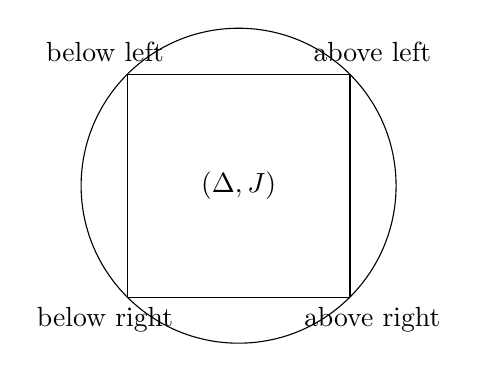
\begin{tikzpicture}[scale=2]
    % Draw the circle
    \draw (0,0) circle (1);
    
    % Label the points
    \foreach \i/\j in {1/above left, 2/below left, 3/below right, 4/above right} {
        \node at (\i*90-45:1.2) {\j};
    }
    
    % Draw the lines connecting the points
    \draw (1*90-45:1) -- (2*90-45:1);
    \draw (2*90-45:1) -- (3*90-45:1);
    \draw (3*90-45:1) -- (4*90-45:1);
    \draw (4*90-45:1) -- (1*90-45:1);
    
    % Draw the center label
    \node at (0,0) {$(\Delta, J)$};
\end{tikzpicture}

\end{document}